

\tikzset{every picture/.style={line width=0.75pt}} %set default line width to 0.75pt        

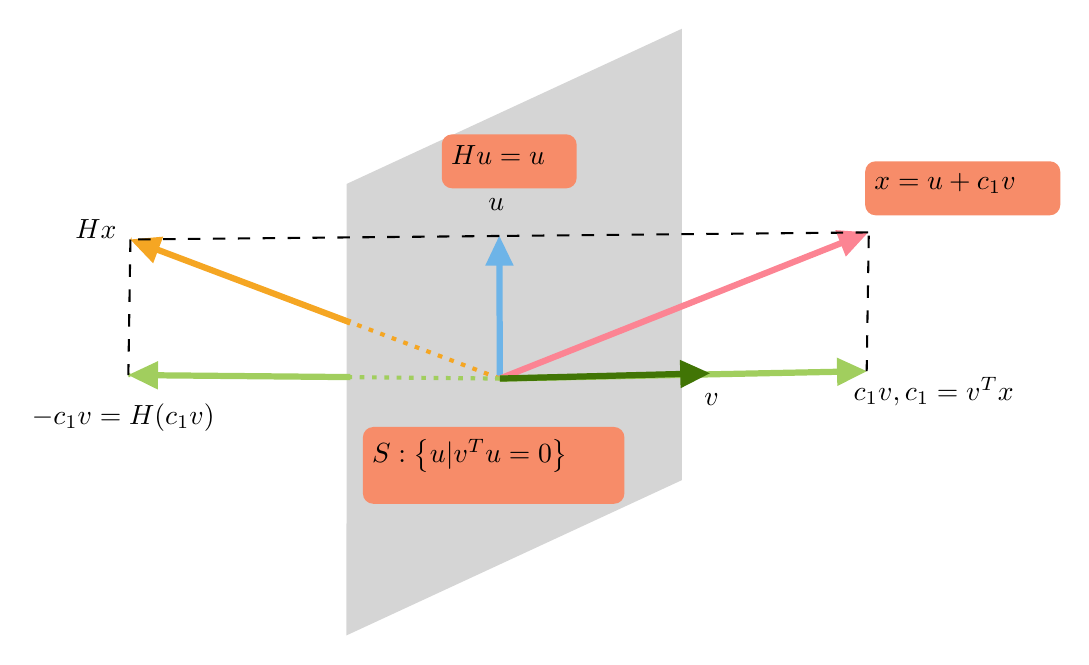
\begin{tikzpicture}[x=0.75pt,y=0.75pt,yscale=-1,xscale=1]
%uncomment if require: \path (0,334); %set diagram left start at 0, and has height of 334

%Shape: Parallelogram [id:dp7838939596356449] 
\draw  [color={rgb, 255:red, 0; green, 0; blue, 0 }  ,draw opacity=0 ][fill={rgb, 255:red, 213; green, 213; blue, 213 }  ,fill opacity=1 ] (401.66,234.62) -- (240.09,309.42) -- (240.16,91.9) -- (401.73,17.11) -- cycle ;
%Straight Lines [id:da6147749821862796] 
\draw [color={rgb, 255:red, 109; green, 180; blue, 232 }  ,draw opacity=1 ][line width=2.25]    (314,185.67) -- (313.74,121.96) ;
\draw [shift={(313.72,116.96)}, rotate = 449.76] [fill={rgb, 255:red, 109; green, 180; blue, 232 }  ,fill opacity=1 ][line width=0.08]  [draw opacity=0] (14.29,-6.86) -- (0,0) -- (14.29,6.86) -- cycle    ;
%Straight Lines [id:da41583656892756826] 
\draw [color={rgb, 255:red, 245; green, 166; blue, 35 }  ,draw opacity=1 ][line width=1.5]  [dash pattern={on 1.69pt off 2.76pt}]  (314,185.67) -- (136,118.67) ;
%Straight Lines [id:da16926502578383218] 
\draw [color={rgb, 255:red, 245; green, 166; blue, 35 }  ,draw opacity=1 ][line width=2.25]    (242,158.67) -- (140.68,120.43) ;
\draw [shift={(136,118.67)}, rotate = 380.66999999999996] [fill={rgb, 255:red, 245; green, 166; blue, 35 }  ,fill opacity=1 ][line width=0.08]  [draw opacity=0] (14.29,-6.86) -- (0,0) -- (14.29,6.86) -- cycle    ;
%Straight Lines [id:da9973542879627482] 
\draw [color={rgb, 255:red, 252; green, 132; blue, 147 }  ,draw opacity=1 ][line width=2.25]    (314,185.67) -- (486.78,117.1) ;
\draw [shift={(491.43,115.25)}, rotate = 518.35] [fill={rgb, 255:red, 252; green, 132; blue, 147 }  ,fill opacity=1 ][line width=0.08]  [draw opacity=0] (14.29,-6.86) -- (0,0) -- (14.29,6.86) -- cycle    ;
%Straight Lines [id:da33840798922577653] 
\draw [color={rgb, 255:red, 161; green, 206; blue, 94 }  ,draw opacity=1 ][line width=1.5]  [dash pattern={on 1.69pt off 2.76pt}]  (314,185.67) -- (135,183.96) ;
%Straight Lines [id:da7106398441661397] 
\draw [color={rgb, 255:red, 161; green, 206; blue, 94 }  ,draw opacity=1 ][line width=2.25]    (242,184.96) -- (140,184.01) ;
\draw [shift={(135,183.96)}, rotate = 360.53999999999996] [fill={rgb, 255:red, 161; green, 206; blue, 94 }  ,fill opacity=1 ][line width=0.08]  [draw opacity=0] (14.29,-6.86) -- (0,0) -- (14.29,6.86) -- cycle    ;
%Straight Lines [id:da3197102975021888] 
\draw [color={rgb, 255:red, 161; green, 206; blue, 94 }  ,draw opacity=1 ][line width=2.25]    (314,185.67) -- (485.73,182.21) ;
\draw [shift={(490.73,182.11)}, rotate = 538.85] [fill={rgb, 255:red, 161; green, 206; blue, 94 }  ,fill opacity=1 ][line width=0.08]  [draw opacity=0] (14.29,-6.86) -- (0,0) -- (14.29,6.86) -- cycle    ;
%Straight Lines [id:da07789590448724115] 
\draw  [dash pattern={on 4.5pt off 4.5pt}]  (136,118.67) -- (135,183.96) ;
%Straight Lines [id:da5486690595919534] 
\draw  [dash pattern={on 4.5pt off 4.5pt}]  (313.72,116.96) -- (136,118.67) ;
%Straight Lines [id:da1919773551202424] 
\draw  [dash pattern={on 4.5pt off 4.5pt}]  (491.43,115.25) -- (313.72,116.96) ;
%Straight Lines [id:da06488229558680647] 
\draw  [dash pattern={on 4.5pt off 4.5pt}]  (491.73,116.81) -- (490.99,164.67) -- (490.73,182.11) ;
%Straight Lines [id:da5187220488118582] 
\draw [color={rgb, 255:red, 65; green, 117; blue, 5 }  ,draw opacity=1 ][line width=2.25]    (314,185.67) -- (410.18,183.23) ;
\draw [shift={(415.18,183.11)}, rotate = 538.55] [fill={rgb, 255:red, 65; green, 117; blue, 5 }  ,fill opacity=1 ][line width=0.08]  [draw opacity=0] (14.29,-6.86) -- (0,0) -- (14.29,6.86) -- cycle    ;

% Text Node
\draw (108,107.4) node [anchor=north west][inner sep=0.75pt]    {$\boldsymbol{Hx}$};
% Text Node
\draw (307,97.4) node [anchor=north west][inner sep=0.75pt]    {$u$};
% Text Node
\draw  [color={rgb, 255:red, 12; green, 12; blue, 12 }  ,draw opacity=0 ][fill={rgb, 255:red, 247; green, 140; blue, 105 }  ,fill opacity=1 ]  (286,73) .. controls (286,70.24) and (288.24,68) .. (291,68) -- (346,68) .. controls (348.76,68) and (351,70.24) .. (351,73) -- (351,89) .. controls (351,91.76) and (348.76,94) .. (346,94) -- (291,94) .. controls (288.24,94) and (286,91.76) .. (286,89) -- cycle  ;
\draw (289,72) node [anchor=north west][inner sep=0.75pt]   [align=left] {$\displaystyle \boldsymbol{Hu=u}$};
% Text Node
\draw (87,196.4) node [anchor=north west][inner sep=0.75pt]    {$\boldsymbol{-c_{1} v=H( c_{1} v)}$};
% Text Node
\draw  [color={rgb, 255:red, 0; green, 0; blue, 0 }  ,draw opacity=0 ][fill={rgb, 255:red, 247; green, 140; blue, 105 }  ,fill opacity=1 ]  (490,86) .. controls (490,83.24) and (492.24,81) .. (495,81) -- (579,81) .. controls (581.76,81) and (584,83.24) .. (584,86) -- (584,102) .. controls (584,104.76) and (581.76,107) .. (579,107) -- (495,107) .. controls (492.24,107) and (490,104.76) .. (490,102) -- cycle  ;
\draw (493,85.4) node [anchor=north west][inner sep=0.75pt]    {$\boldsymbol{x=u+c_{1} v}$};
% Text Node
\draw  [color={rgb, 255:red, 0; green, 0; blue, 0 }  ,draw opacity=0 ][fill={rgb, 255:red, 247; green, 140; blue, 105 }  ,fill opacity=1 ]  (248,214) .. controls (248,211.24) and (250.24,209) .. (253,209) -- (369,209) .. controls (371.76,209) and (374,211.24) .. (374,214) -- (374,241) .. controls (374,243.76) and (371.76,246) .. (369,246) -- (253,246) .. controls (250.24,246) and (248,243.76) .. (248,241) -- cycle  ;
\draw (251,213.4) node [anchor=north west][inner sep=0.75pt]    {$S:\left\{\boldsymbol{u} |\boldsymbol{v}^{T}\boldsymbol{u} =0\right\}$};
% Text Node
\draw (483,183.4) node [anchor=north west][inner sep=0.75pt]    {$\boldsymbol{c_{1} v} ,\boldsymbol{c_{1} =v}^{T}\boldsymbol{x}$};
% Text Node
\draw (411,191.4) node [anchor=north west][inner sep=0.75pt]    {$\boldsymbol{v}$};


\end{tikzpicture}